\documentclass[twocolumn]{article}

\usepackage{amsmath, amssymb} % Math formatting and symbols
\usepackage{graphicx} % Insert graphics
\usepackage{wrapfig} % Allow text to wrap around images
\usepackage[cm]{fullpage} % Smaller margins and header/footer
\usepackage{setspace}
\usepackage{gensymb} % degree symbol
\usepackage{graphicx} % Insert graphics
\usepackage{wrapfig} % Allow text to wrap around images
\usepackage{amsmath, amssymb} % Math formatting and symbols
\usepackage{graphicx} % Insert graphics
\usepackage{wrapfig} % Allow text to wrap around images
\usepackage[cm]{fullpage} % Smaller margins and header/footer
\usepackage{setspace}
\usepackage{gensymb} % degree symbol

\usepackage{float}

\usepackage{enumitem} % Allow for widest tag in enumerate

\usepackage{enumitem} % Allow for widest tag in enumerate

\renewcommand*\descriptionlabel[1]{\hspace\leftmargin$#1$}

\newenvironment{adescription}[1]
{\begin{list}{}%
		{\renewcommand\makelabel[1]{##1\hfill}%
			\settowidth\labelwidth{\makelabel{#1}}%
			\setlength\leftmargin{\labelwidth}
			\addtolength\leftmargin{\labelsep}}}
	{\end{list}}

\newcommand{\bd}{\textbf}
\newcommand{\dquad}{\quad{}\quad{}}

\title{Graph of Equations}
\author{}
\date{}

\begin{document}
	\setstretch{0.5}
	\maketitle{}
	
	\section{Review}
	Assume...
	\begin{adescription}{\dquad{}$P_2$:}
		\item[\dquad{}$P_1$:] $(x_1, y_1)$
		\item[\dquad{}$P_2$:] $(x_2, y_2)$
	\end{adescription}
	%		\begin{adescription}{\dquad{}$(x_2, y_2)$:}
	%			\item[\dquad{}$(x_1, y_1)$:] Point 1
	%			\item[\dquad{}$(x_2, y_2)$:] Point 2
	%		\end{adescription}
	\subsection{Distance Formula}
	\begin{equation*}
		d = \sqrt{(x_2 - x_1)^2 + (y_2 - y_1)^2}
	\end{equation*}
	where:
	\begin{adescription}{\dquad{}$d$:}
		\item[\dquad{}$d$:] Distance between $P_1$ and $P_2$
	\end{adescription}
	
	\subsection{The Midpoint Formula}
	\begin{equation*}
		m = (\frac{x_1+x_2}{2}, \frac{y_1+y_2}{2})
	\end{equation*}
	where:
	\begin{adescription}{\dquad{}$m$:}
		\item[\dquad{}$m$:] Midpoint between $P_1$ and $P_2$
	\end{adescription}
	
	\section{Equations of Circles}
	You can draw a circle using an \bd{relationship} not a function.
	\begin{equation*}
		(x - h)^2 + (y - k)^2 = r^2
	\end{equation*}
	where:
	\begin{adescription}{\dquad{}$(h, k)$:}
		\item[\dquad{}$(h, k)$:] Center Point
		\item[\dquad{}$r$:] Radius
	\end{adescription}
	
	\section{Symmetry}
	\subsection{Y-Axis}
	\begin{itemize}[label=\dquad{}--]
		\item Called an "\bd{Even Function}"
		\item Looks the same after reflection over Y-Axis
		\item Has to meet the following requirement(s)...
	\end{itemize}
	\begin{equation*}
		f(x) = f(-x)
	\end{equation*}
	\par One example of such a function is $y = x^2$.
	\begin{align*}
		f(4) &= 16 \\
		f(-4) &= 16 \\
		16 &= 16
	\end{align*}
	
	\subsection{X-Axis}
	\begin{itemize}[label=\dquad{}--]
		\item \bd{Not a function}, doesn't pass vertical line test
		\item Called a \bd{relationship}
		\item Has to meet the following requirement(s)...
	\end{itemize}
	\begin{equation*}
		x \mapsto \{-y,  y\}
	\end{equation*}
	One example of such a equation is $x = y^2$ but \bd{not} $y = \sqrt{x}$ because that would only allow positive x values.
	\begin{align*}
		9^2 &= 81 \\
		(-9)^2 &= 81
	\end{align*}
	
	\subsection{Origin}
	\begin{itemize}[label=\dquad{}--]
		\item Called an "\bd{Odd Function}"
		\item Visually the same after $180\degree{}$ rotation about $(0, 0)$
		\item Has to meet the following requirement(s)...
	\end{itemize}
	\begin{align*}
		f(x) &= y \\
		f(-x) &= -y
	\end{align*}
	One example of such a function is $y = x^3$
	\begin{align*}
		f(2) &= 8 \\
		f(-2) &= -8
	\end{align*}
	
	\section{Equations of  Lines}
	Assume...
	\begin{adescription}{\dquad{}$P_2$:}
		\item[\dquad{}$m$:] Slope
	\end{adescription}
	\subsection{Slope}
	You can use the slope formula to find the rate of change between two points.
	\begin{equation*}
		m = \frac{\text{"Ryse"}}{\text{Run}} = \frac{y_2-y_1}{x_2-x_1}
	\end{equation*}
	\subsection{Forms}
	\subsubsection{Slope-Intercept Form}
	\begin{equation*}
		y = mx + b
	\end{equation*}
	where:
	\begin{adescription}{\dquad{}$b$:}
		\item[\dquad{}$b$:] x-intercept
	\end{adescription}
	\subsubsection{Point Slope Form}
	If you need point-slope form, just sub out values. However, if you need to find slope-intercept form you can solve for $y$.
	\begin{equation*}
		y - y_1 = m(x - x_1)
	\end{equation*}
	\subsubsection{Intercept Form}
	\begin{equation*}
		\frac{x}{a} + \frac{y}{b} = 1
	\end{equation*}
	where:
	\begin{adescription}{\dquad{}$b$:}
		\item[\dquad{}$a$:] x-intercept, point (a, 0) falls on the line
		\item[\dquad{}$b$:] y-intercept, point (0, b) falls on the line
	\end{adescription}
	This form can be converted into \bd{General Form} through the multiplication of the least common multiple of $a$ and $b$. Then subtracting   the value on the right side of the equation.
	\subsubsection{General Form}
	\begin{equation*}
		Ax + By + C = 0
	\end{equation*}
	where:
	\begin{itemize}[label=--]
		\item[] $A$ is non-negative
		\item[] $A$, $B$, and $C$ are all \emph{integers}
	\end{itemize}
	\subsection{Relationships of Lines}
	\subsubsection{Parallel Lines}
	-- \bd{same slopes}.
	\subsubsection{Perpendicular Lines}
	-- \bd{opposite reciprocal slopes}. \\
	Consider the following where lines $t_1$ and $t_2$ are perpendicular.
	\begin{align*}
		t_1 &= 3/8 \\
		t_2 &= -8/3
	\end{align*}
	
	\section{Functions and Equations}
	
	\subsection{Is it a function?}
	-- Each $x$ only maps to one $y$
	
	\section{Domain \& Range}
	
	\subsection{Formatting}
	Example...
	\begin{align*}
		D&: (-1,2] \\
		R&: (-\infty, 12)
	\end{align*}
	\begin{itemize}[label=--]
		\item "(", ")" means exclusive
		\item "[", "]" means inclusive
		\item \bd{Never} use [] with $\infty$
	\end{itemize}
	
	\subsection{Zeros}
	Solve for when $y = 0$ \\
	They are x-intercepts
	
	\subsection{Increasing and Decreasing}
	\par \bd{Never} use "[", "]", always "(", ")" \\
	\bd{Always} Least $\to$ Greatest \\
	
	
	\subsection{Relative Maximum and Minimum}
	A \bd{point} on a line where the line is either above on both sides (\emph{Minimum}) or below on both sides (\emph{Maximum}). \bd{Cannot} be an \bd{end point}.
	
	
	\subsection{New Functions}
	
	\subsubsection{Greatest Integer Function (Floor)}
	Represented by
	\begin{equation*}
		f(x) = [[x]]
	\end{equation*}
	
	Left side solid (\emph{Included}), right side empty (\emph{Excluded})
	
	\subsubsection{Peace-wise Function}
	\par An equation, but with conditionals
	
	Example...
	\begin{align*}
		f(x) = 
		\begin{cases}
			x^2 - 3      &\quad \text{if } x \ge 3 \\
			-2x^4 + 9x^3 &\quad \text{if } x < 3
		\end{cases}
	\end{align*}
	
	Plug it into calculator by multiplying things and conditions
	
	\begin{equation*}
		f(x) = (x^2 - 3)(x \ge 3) + (-2x^4 + 9x^3)(x < 3)
	\end{equation*}
	
	\subsection{Algebra of functions}
	
	Assume...
	\begin{adescription}{\dquad{}$g(x)$:}
		\item[\dquad{}$f(x)$:] 3x + 1
		\item[\dquad{}$g(x)$:] 4x - 1
	\end{adescription}
	
	\noindent{} Can be done in 2 different ways
	\begin{itemize}
		\item[--] Do the algebra on the function
		\item[--] Do the algebra on the return from the function
	\end{itemize}
	\dquad{}\quad{}-- Only one example will be shown, but it works on them all
	
	\subsubsection{Addition of functions}
	Algebra on the functions...
	\begin{align*}
		h(x) &= (f + g)(x) \\
		&= 3x + 3 + 4x - 1 \\
		&= 7x + 2
	\end{align*}
	Algebra on the return values... (\emph{Only example})
	\begin{align*}
		(f + g)(2) &= f(2) + g(2) \\
		&= (2(2) + 3) + (4(2) - 1) \\
		&= 16
	\end{align*}
	
	\subsubsection{Subtraction of functions}
	\begin{align*}
		h(x) &= (f - g)(x) \\
		&= (3x + 1) - (4x - 1) \\
		&= 3x + 1 - 4x + 1 \\
		&= -x + 2
	\end{align*}
	
	\subsubsection{Multiplication of functions}
	\begin{align*}
		h(x) &= (f * g)(x) \\
		&= (3x + 1)(4x - 1) \\
		&= 12x^2 - 3x + 4x - 1 \\
		&= 12x^2 + x - 1
	\end{align*}
	
	\subsubsection{Division of functions}
	\begin{align*}
		h(x) &= (\frac{f}{g})(x) \\
		&= \frac{3x + 1}{4x - 1}
	\end{align*}
	
	\subsubsection{Composition of functions}
	\begin{align*}
		h(x) &= (f \circ g)(x) = f(g(x)) \\
		&= 3(4x - 1) + 1 \\
		&= 12x - 3 + 1 \\
		&= 12x - 2
	\end{align*}
	
	\subsubsection{Inverse of functions}
	Swap the $x/y$ values and then solve for $y$;
	
	\begin{align*}
		y &= 3x + 1
		\intertext{Swap the x and y} \\
		x &= 3y + 1 \\
		3y &= x - 1 \\
		y &= \frac{x - 1}{3}
	\end{align*}

	\setstretch{1}
\maketitle{}

\subsection*{How to answer questions}

Evaluate the trigonometric functions of the quadrant angle, if possible \\
\indent -- Radians

\noindent Reference Angle \\
\indent -- Degrees/Radians will be specified \\
\indent -- Always acute \\
\indent -- Always positive \\
\indent -- Between x-axis and terminal side

\noindent Find two solutions of the equation. Give your answers in degrees ($ 0^\circ \le \theta < 360^\circ $) and in radians ($ 0 \le \theta < 2\pi $). Do not use a calculator. $ \sin(\theta) = -\frac{1}{2} $ \\
\indent -- Always positive \\
\indent -- Two answers \\
\indent -- Exact values, draw circle

\noindent Find the value of the expression, if possible $ \sin^{-1}(-\frac{\sqrt{3}}{2}) \text{ or}  \arcsin(-\frac{\sqrt{3}}{2}) $ \\
\indent -- Radians assumed, unless specified otherwise \\
\indent -- Exact = Picture, Round = Calculator \\
\indent -- Positive or negative

\subsection*{Basic Trigonometric Functions}
\begin{align*}
	sin &= \frac{y}{r}  & csc &= \frac{r}{y} \\
	cos &= \frac{x}{r} & sec &= \frac{r}{x} \\
	tan &= \frac{y}{x} & cot &= \frac{x}{y}
\end{align*}

\begin{figure}[h]
	\centering
	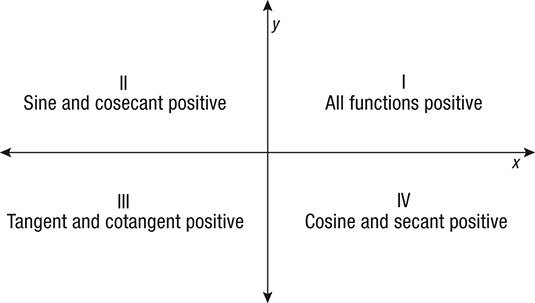
\includegraphics[width=0.25\textwidth]{positive_quadrants.jpg}
\end{figure}

\subsection*{Graphing Trigonometric Functions}

Assume...
\begin{itemize}[label=--]
	\setlength\itemsep{-0.55em}
	\item $ y = d + a * trig(bx - c) $
	\item Amplitude = $ \vert a \vert $
	\item Vertical Shift = $d$
	\item Phase Shift = $ \frac{c}{b} $
	\item X-Scale (change between critical points) = $ \frac{\text{period}}{4} $
	\item Period depends on what functions
	\item sin, cos, csc, sec = $ \frac{2\pi}{b} $
	\item tan, cot = $ \frac{\pi}{b} $
\end{itemize}
For deriving from a word problem
\begin{itemize}[label=--]
	\setlength\itemsep{-0.55em}
	\item $ c = b * \text{shift} $
	\item b depends on what functions
	\item sin, cos, csc, sec = $ \frac{2\pi}{\text{period}} $
	\item tan, cot = $ \frac{\pi}{\text{period}} $
\end{itemize}

\subsubsection*{Examples...}

\begin{figure}[H]
	\centering
	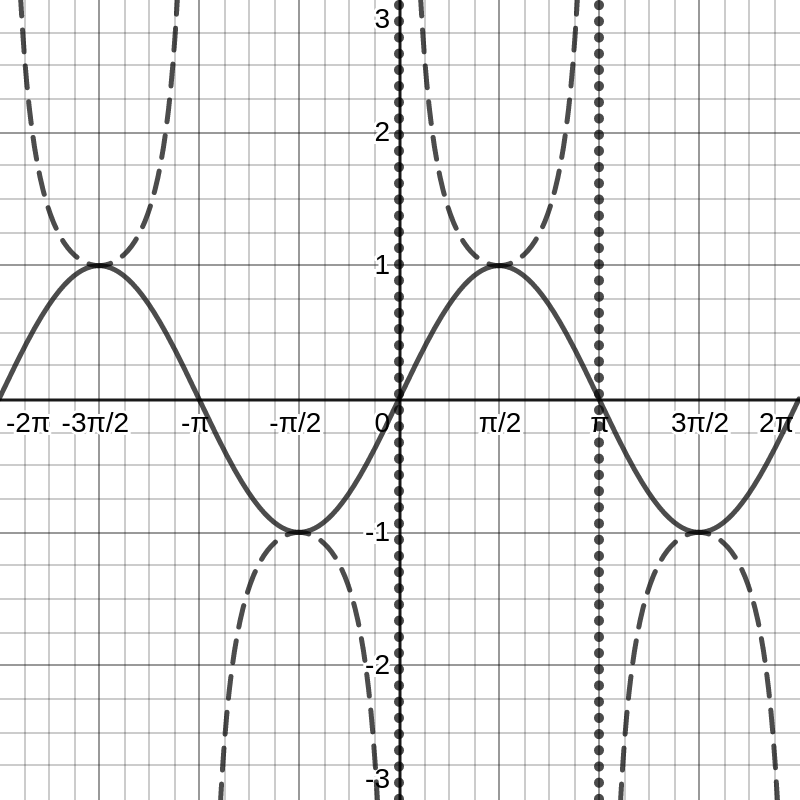
\includegraphics[width=0.20\textwidth]{sin-csc.png}
	\caption{$ y = \sin(x), y = \csc(x) $}
\end{figure}

\begin{figure}[H]
	\centering
	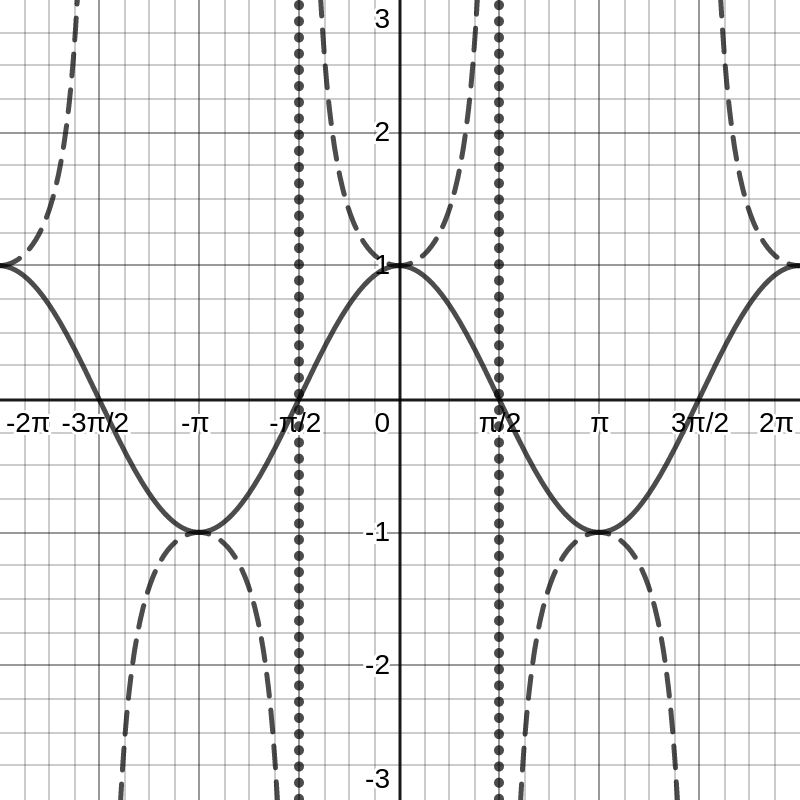
\includegraphics[width=0.20\textwidth]{cos-sec.png}
	\caption{$ y = \cos(x), y= \sec(x) $}
\end{figure}

\begin{figure}[H]
	\centering
	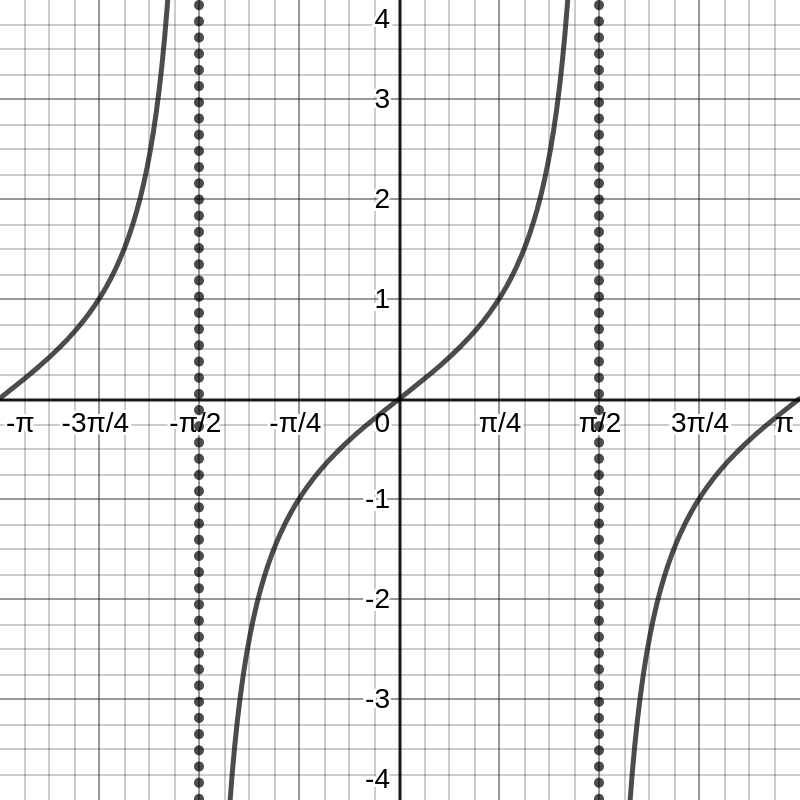
\includegraphics[width=0.20\textwidth]{tan.png}
	\caption{$ y = \tan(x) $}
\end{figure}

\begin{figure}[H]
	\centering
	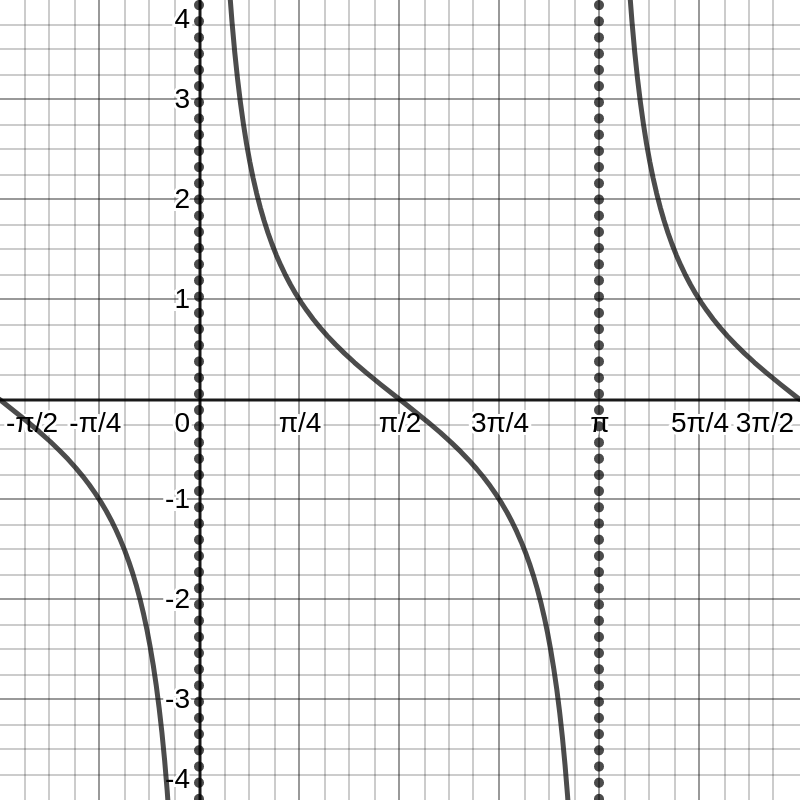
\includegraphics[width=0.20\textwidth]{cot.png}
	\caption{$ y = \cot(x) $}
\end{figure}

\subsection*{Trigonometric Identities}

\begin{align*}
	\sin &= \frac{1}{\csc}  & \csc & = \frac{1}{\sin} \\
	\cos &= \frac{1}{\sec} & \sec & = \frac{1}{\cos} \\
	\tan &= \frac{\sin}{\cos}  & \cot & = \frac{\cos}{\sin}
\end{align*}
\vspace{0pt}
\begin{align*}
	\sin^2 + \cos^2 &= 1 \\
	1 + \tan^2 &= \sec^2 \\
	1 + \cot^2 &= \csc^2
\end{align*}
\vspace{-2.2em}
\subsection*{Arcs}
In \bd{radians} unless specified otherwise \\
Exact $\implies$ picture \\
Round $\implies$ calculator ($\sin^{-1}$)

\begin{align*}
	\sin(\theta) = -\frac{\sqrt{3}}{2} \\
	\sin^{-1}(-\frac{\sqrt{3}}{2}) \\
	\arcsin(-\frac{\sqrt{3}}{2})
\end{align*}

\begin{figure}[H]
	\centering
	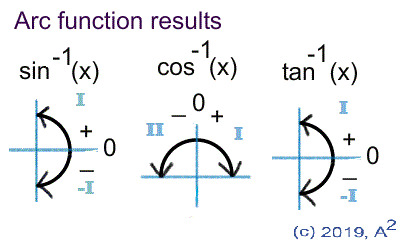
\includegraphics[width=0.20\textwidth]{ArcTrig.jpg}
\end{figure}



\end{document}
